\documentclass[10pt]{amsart}
\usepackage{geometry}                
\geometry{letterpaper}                  
\usepackage[parfill]{parskip}    
\usepackage{graphicx}
\usepackage{amssymb}
\usepackage{epstopdf}
\usepackage{subfigure}
\DeclareGraphicsRule{.tif}{png}{.png}{`convert #1 `dirname #1`/`basename #1 .tif`.png}
\evensidemargin=0in
\oddsidemargin=0in

\title{ECE 532 Final Project: Voltage Regulator}
\author{John O'Hollaren}

\begin{document}
\maketitle

%%%%%%%%%%%%%%%%%%%%%%%%%%%%%%%%%%%%%%%%%%%%%
\section{Introduction}
In this report I will detail the design of a linear regulator that takes a 5 volt input and outputs 1.0 - 4.0 volts on the output. I can control it by tuning the feedback amplifiers. I fine tune the final amplifier that will be fabricated to output 2.5V. I learned a lot in this project, from how to design a negative feedback controller to the design tradeoffs involved in analog circuits. Almost every decision I made had a pro and a con (such as more current vs. using more area). The layout showed me how important it is to plan ahead and think of a project modularly.

This report is divided into the following sections:
\begin{enumerate}
\item Design Goals
\item Design Challenges
\item Schematics
\item Simulations
\item Layout
\end{enumerate}

	\begin{center}
		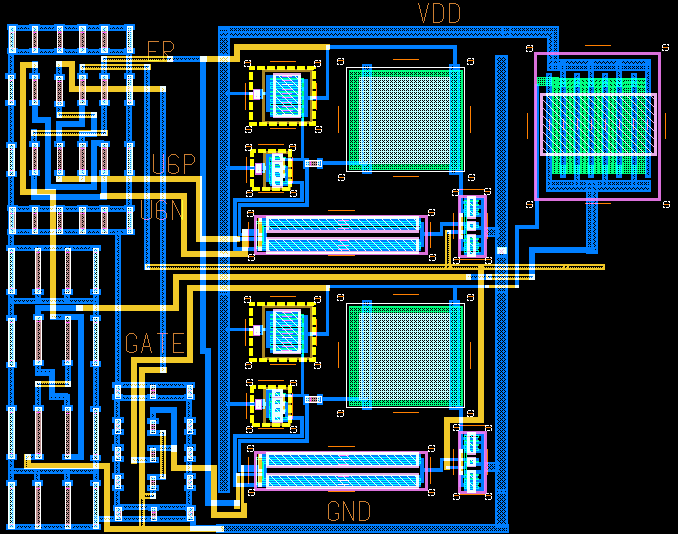
\includegraphics[width=4in]{Media/lay_final.png}
	\end{center}

\newpage

%%%%%%%%%%%%%%%%%%%%%%%%%%%%%%%%%%%%%%%%%%%%%
\section{Design Goals}

There are several types of linear regulators. Note that drop out depends on a variety of factors, not just the topology (as I show later). My design will use only one power element, and thus falls under the LDO category with a minimum drop of 1 Volt.

\begin{figure}[h]
	\begin{center}
		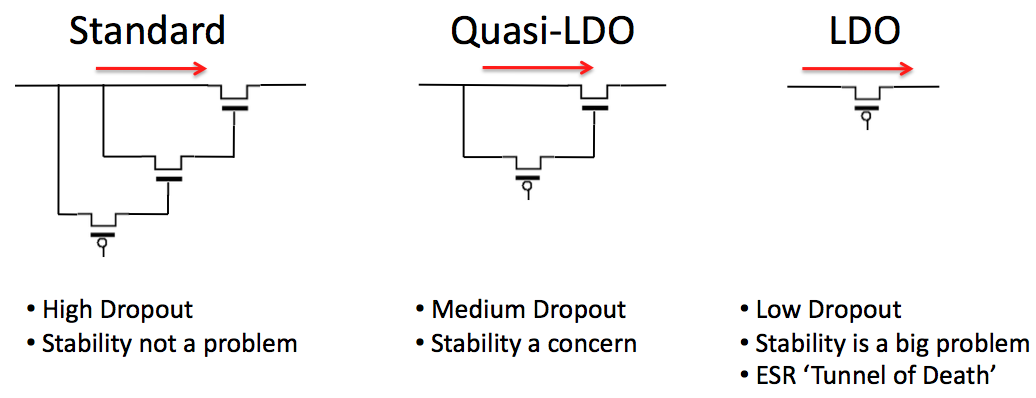
\includegraphics[width=6in]{Media/ldos.png}
	\end{center}
	\caption{Comparison of linear regulator topologies}
	\label{fig:wl}
\end{figure}

I have cut down significantly on the amount of I/O, external power, and references needed from my earlier, more complicated designs. Here is a black box I/O diagram of my final design: 

\begin{figure}[h]
	\begin{center}
		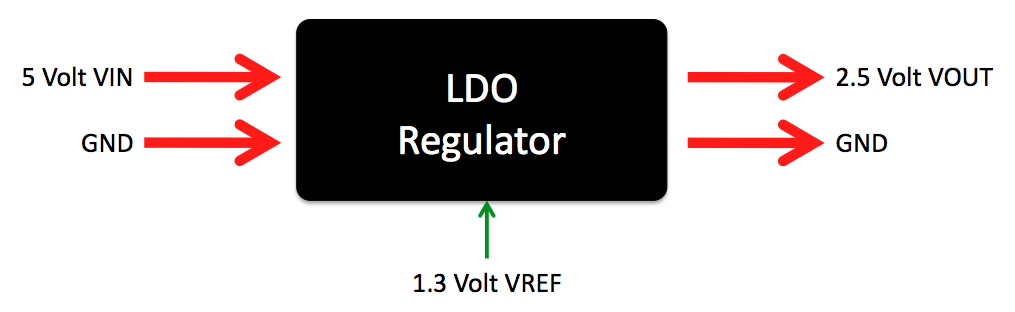
\includegraphics[width=6in]{Media/black.png}
	\end{center}
	\caption{I/O Diagram}
	\label{fig:black}
\end{figure}

Following are the specifications I am designing to. For comparison, I am using the Texas Instruments TLV1171 which is a highly optimized linear regulator that claims 500x lower quiescent power draw over most commercial regulators.

\begin{figure}[h]
	\begin{center}
		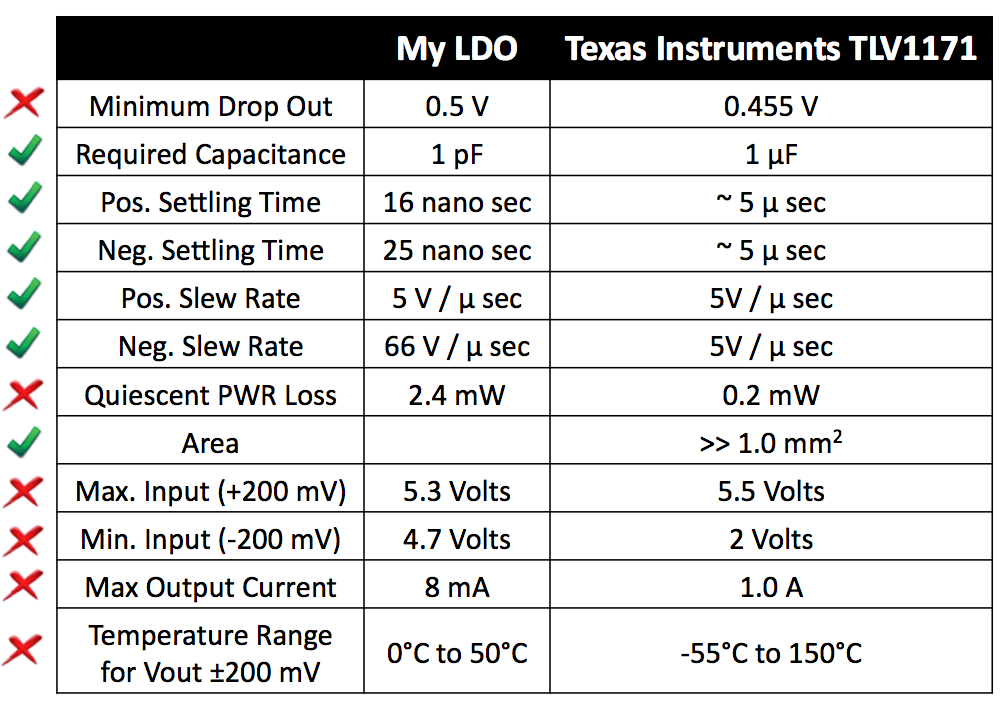
\includegraphics[width=6in]{Media/specs.png}
	\end{center}
	\caption{I/O Diagram. Specs from Texas Instruments's part I am able to match or beat are highlighted with green; specs I am not able to match are marked with red.}
	\label{fig:specs}
\end{figure}

%%%%%%%%%%%%%%%%%%%%%%%%%%%%%%%%%%%%%%%%%%%%%
\section{Design Challenges}

There are a few key challenges I must work around to design this linear regulator. These include a physical limitation with the power MOSFET and process limitations (limited voltage range).

\subsection{Power MOSFET Limitations}

The rule of thumb for analog amplifier design is:
\begin{equation}
\text{Max } I_{DS} = \frac{1 \text{mA}}{ 1 \mu m}
\end{equation}

This suggests that I find the ideal $\frac{W}{L}$ ratio and then scale it up to the current I need. However, there is a problem. As $\frac{W}{L}$, decreases, the $V_{DS}$ of the mosfet becomes a bigger factor. In order to have an efficient regulator, I need a very high $\frac{W}{L}$, which costs a lot of area that I do not have. On the flip side, a larger ratio decreases the size of the controllable linear region, which makes the regulator harder to control. The best compromise, is L = 8u, W = 420 u as shown in Figure \ref{fig:wl}.

I want to find a linearization point for my feedback circuit with a large linear region. The middle graph is ideal for this. So my power MOSFET pass element will have $\frac{W}{L}=\frac{420}{8}=\frac{52.5}{1}$ which will allow up to 8mA of output current.

\begin{figure}[h]
	\begin{center}
		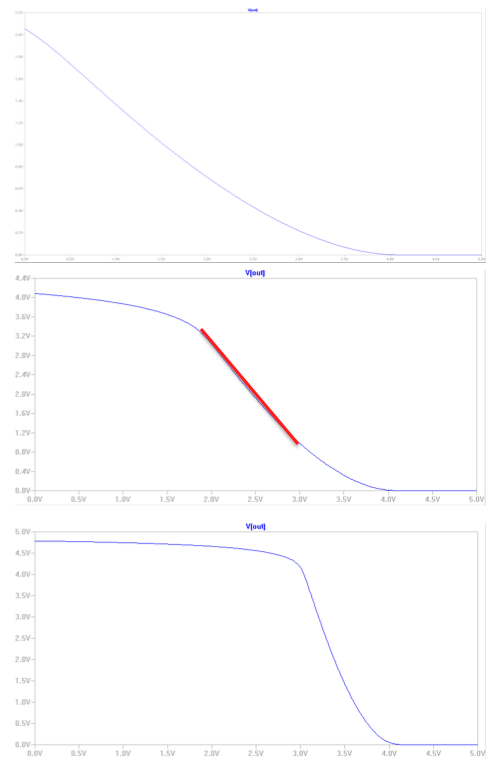
\includegraphics[width=4.0in]{Media/WL.png}
	\end{center}
	\caption{L = 8u for all. Top: W = 100u, Middle: W = 420u, Bottom: W = 1000u. $V_{DS}$ vs $V_{GS}$ for a single MOSFET using our technology. This is an important graph because $V_{DS}$ determines the output voltage and $V_{GS}$ is what I use to control it. Note the nice linear region in the middle one.}
	\label{fig:wl}
\end{figure}


\subsection{Process Limitation: No Negative Voltage}

Use of the negative voltage rail allows a PID controller to be directly implemented in the feedback path. A negative voltage allows me to create an op amp differentiator around a zero point, so that a $V_{out}$ that is too high can directly cause a gate voltage to compensate. My initial design assumed I had access to this negative voltage, so my controller looked like Figure \ref{fig:piedmont}: \\

\begin{figure}[h]
	\begin{center}
		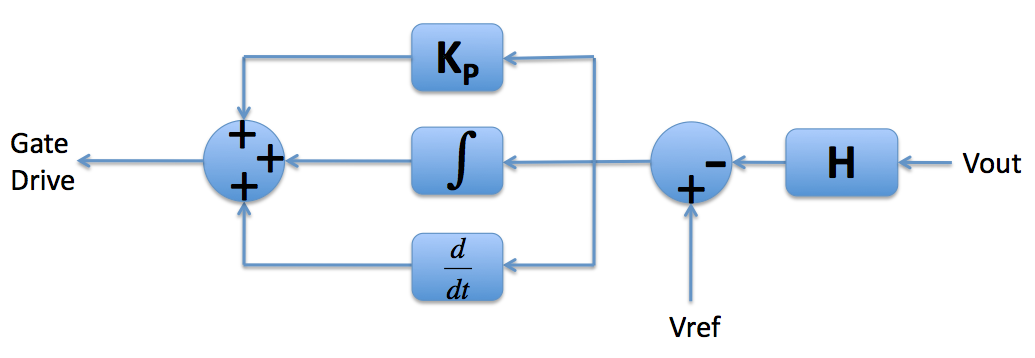
\includegraphics[height=1in]{Media/PID.png}
	\end{center}
	\caption{The initial PID controller I designed.}
	\label{fig:piedmont}
\end{figure}

\begin{figure}[h]
	\begin{center}
		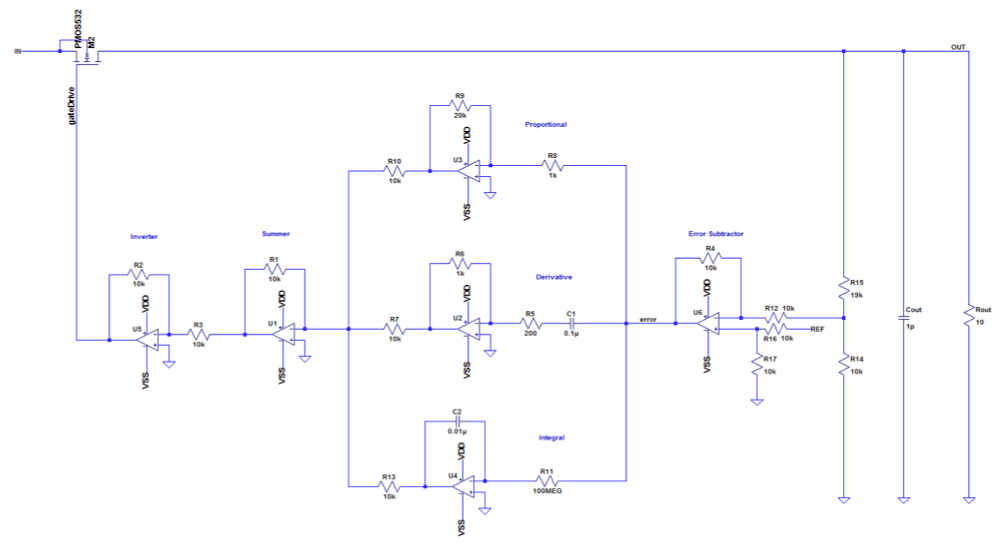
\includegraphics[height=1.7in]{Media/PID_sc.png}
	\end{center}
	\caption{Using this, I can precisely control the output.}
	\label{fig:pid}
\end{figure}

\begin{figure}[h]
	\begin{center}
		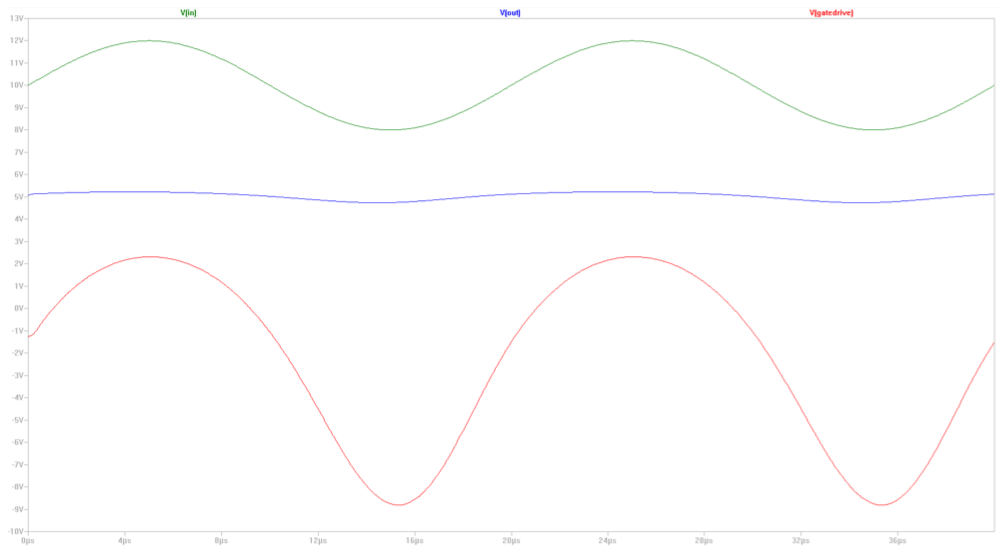
\includegraphics[width=3in]{Media/pidfb.png}
	\end{center}
	\caption{PID controlled output voltage (blue) with a 4V sinusoidal input (green) and the PID controller output (red) to precisely control the blue output and keep it constant.}
	\label{fig:pidfb}
\end{figure}

\newpage

However, to fabricate my design I will need to have a maximum voltage differential on chip of 5V. Therefore, I do not have access to this negative voltage rail, and I will have to improvise with a negative feedback differential amplifier that never pushes the error signal below 0. \\

My solution is to reduce the feedback path to a porportional-only controller, and then use the same reference as I am already using for the op-amps, which is 1.3 Volts. With a 2 Volt output, I then have $V_{error} = 0.3$ which drives my gate to give a 2.0 Volt output. I can tune this to provide a 4.0 Volt output and anything in between or down to 1.0 V as well. These are shown later in the simulations.

\begin{figure}[h]
	\begin{center}
		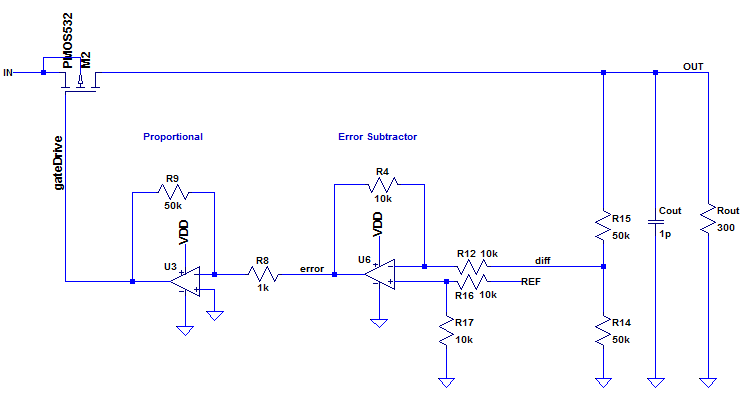
\includegraphics[width=7in]{Media/cleanfinal.png}
	\end{center}
	\caption{A high level view of my final design. Transistor level shown on next page.}
	\label{fig:pidfb}
\end{figure}

\newpage

%%%%%%%%%%%%%%%%%%%%%%%%%%%%%%%%%%%%%%%%%%%%%
\section{Schematics}

Here is the final design:
	\begin{center}
		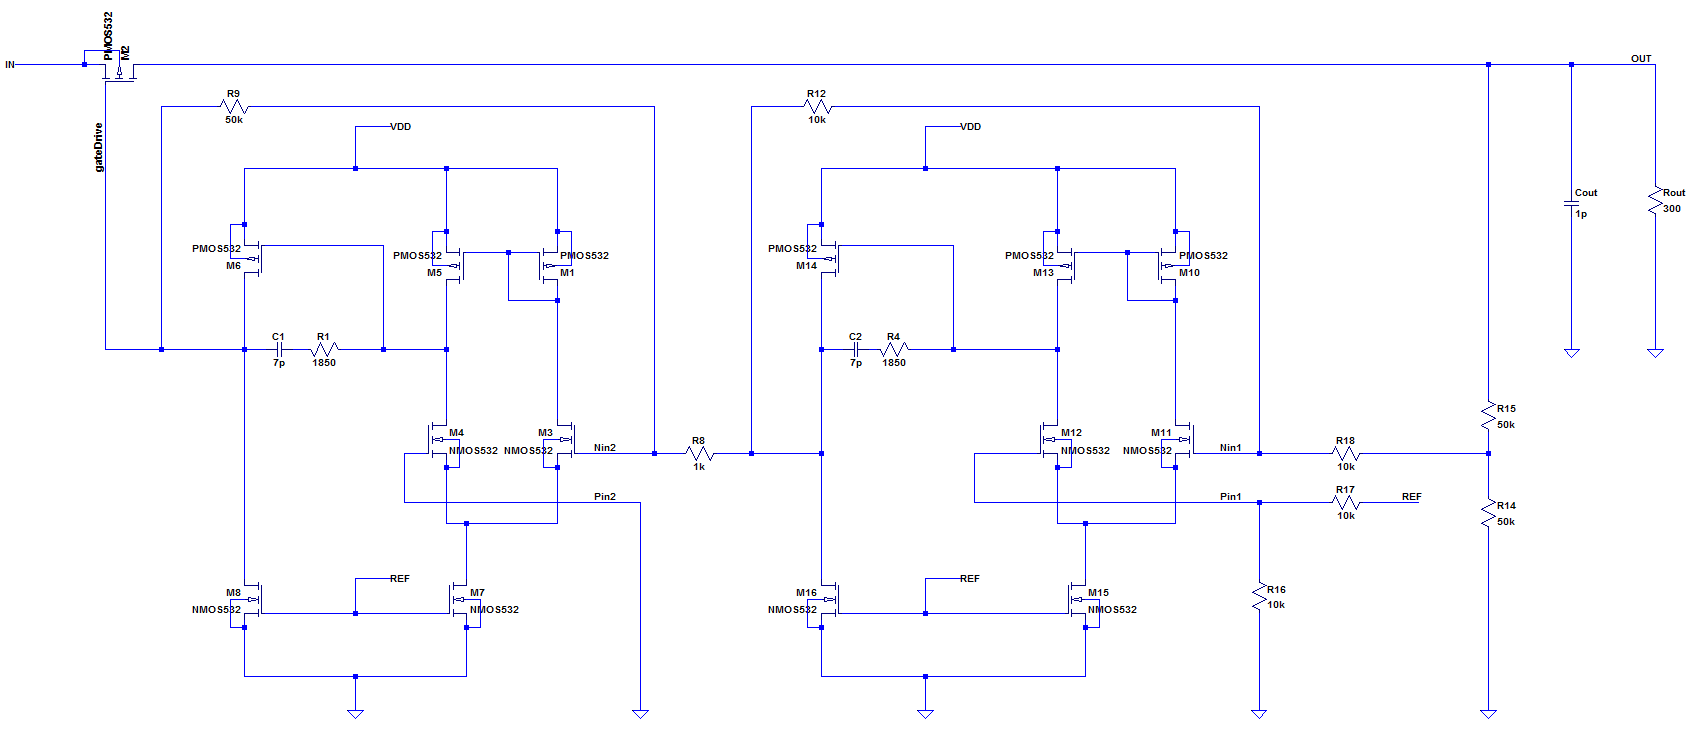
\includegraphics[width=6.0in, angle=90]{Media/design.png}
	\end{center}

\begin{figure}[h]
	\begin{center}
		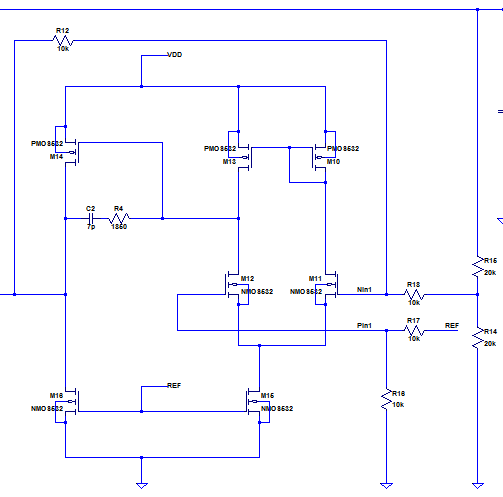
\includegraphics[width=3in]{Media/diff.png}
	\end{center}
	\caption{Close up of differential amplifier.}
	\label{fig:pidfb}
\end{figure}

\begin{figure}[h]
	\begin{center}
		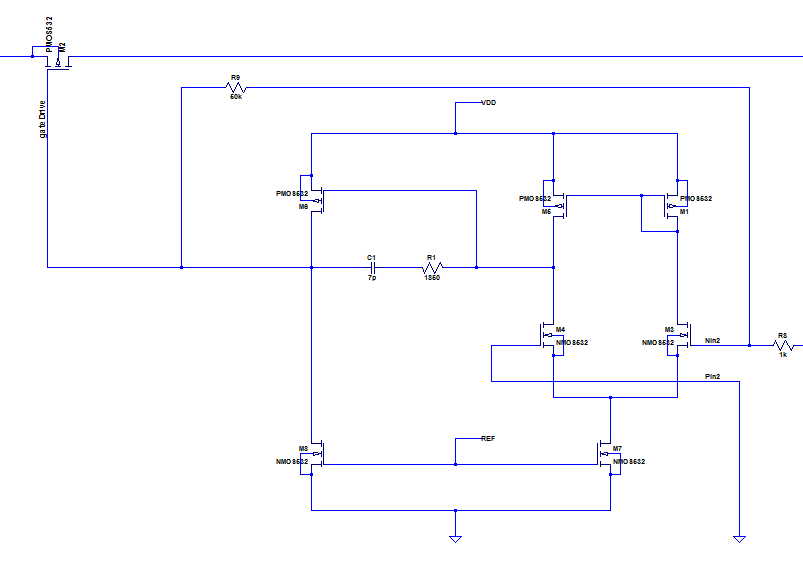
\includegraphics[width=3in]{Media/driver.png}
	\end{center}
	\caption{Close up of gain amplifier and gate driver.}
	\label{fig:pidfb}
\end{figure}

.
\newpage
.
  
%%%%%%%%%%%%%%%%%%%%%%%%%%%%%%%%%%%%%%%%%%%%%
\section{Simulations}

\begin{figure}[h]
	\begin{center}
		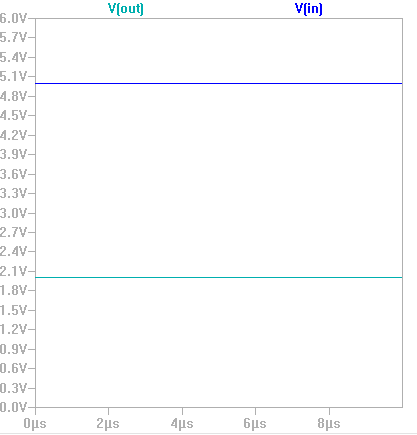
\includegraphics[width=3in]{Media/ss1.png}
	\end{center}
	\caption{Steady State Output. Showing the amplifier tuned for $V_{out} = 2.00$.}
	\label{fig:pidfb}
\end{figure}

\begin{figure}[h]
	\begin{center}
		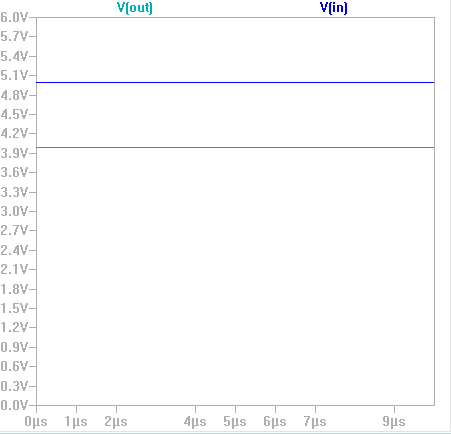
\includegraphics[width=3in]{Media/ss2.png}
	\end{center}
	\caption{Steady State Output. Showing the amplifier tuned for $V_{out} = 4.00$.}
	\label{fig:pidfb}
\end{figure}

Both are accurate in steady state to within 2\%.

\begin{figure}[h]
	\begin{center}
		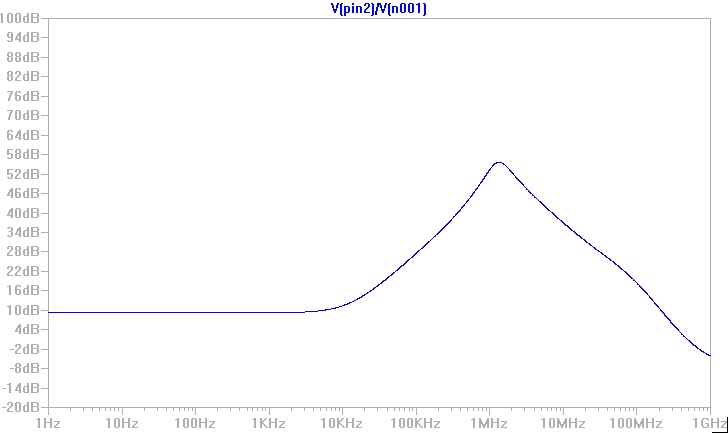
\includegraphics[width=6in]{Media/lg.png}
	\end{center}
	\caption{Loop Gain, $T(s)$.}
	\label{fig:pidfb}
\end{figure}

The loop gain, $T(s)$ is between 10 dB and 60 dB. Note in my previous designs the loop gain was about -20 dB. I have greatly improved it here. This is very import because for a negative feedback voltage regulator we have:\\

\begin{itemize}
\item Voltage noise on the input is rejected in proportion to $\frac{1}{1 + T(s)}$, which is $ \approx 0$ if $T(s)$ is very high.
\item Voltage disturbances on the load are rejected in proportion to $\frac{1}{1 + T(s)}$, which is $ \approx 0$ if $T(s)$ is very high.
\item The reference voltage is followed in proportion to $\frac{T(s)}{1 + T(s)}$, which is $ \approx 1$ if $T(s)$ is very high. \\
\end{itemize}

Therefore, since my loop gain, $T(s)$ is sufficiently high, voltage and current disturbances should be rejected well as they are multiplied by a very small number, and the reference voltage should be followed well as it is multiplied by something close to unity. \\

Note that the above is the idea case; several non-idealities as well as the fact my error amplifier cannot realize the entire negative range will hamper the affect of the feedback circuit to actively compensate.
 
\newpage

The regulator maintains stability even with a sine wave of just under 1 V. The hypothetical noise rejection from the loop gain is not realized, but regulator maintains stability under load.

\begin{figure}[h]
	\begin{center}
		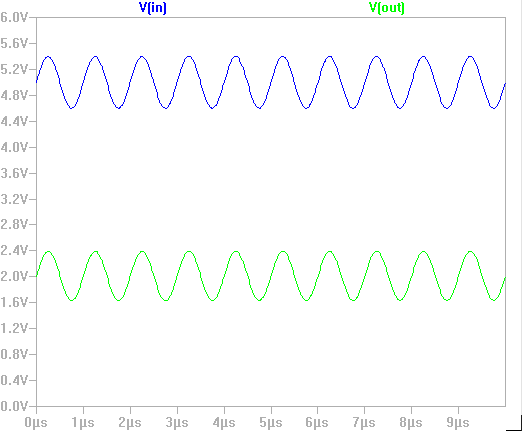
\includegraphics[width=3.5in]{Media/sin.png}
	\end{center}
	\caption{$V_{out} $ vs $V_{in}$ with a sine wave on the input.}
	\label{fig:pidfb}
\end{figure}

Here is the steady state current draw and power loss across the control circuitry:

\begin{figure}[h]
	\begin{center}
		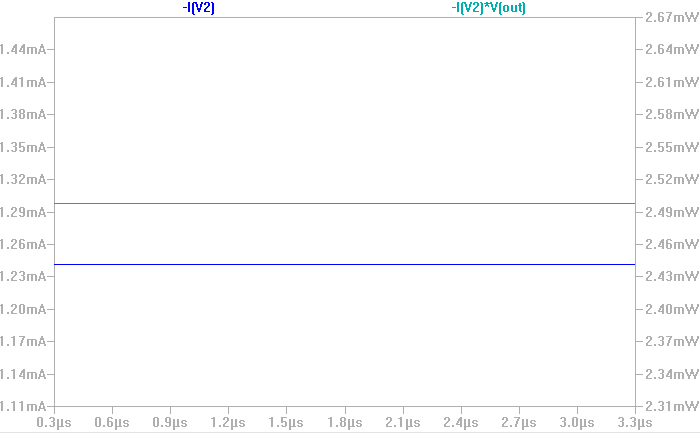
\includegraphics[width=4.5in]{Media/pwr.png}
	\end{center}
	\caption{Steady state current draw and steady state power loss through control circuitry. The quiescent power loss is 2.5 mW.}
	\label{fig:pidfb}
\end{figure}

\newpage

The positive settling time is 10 nano seconds. The negative settling time is 8 nano seconds. From the linear section of the same graphs, I also get the slew rates:

Positive slew rate = \scalebox{1.5}{ $ \frac{100 \text{ Volts}}{\mu \text{ sec}} $ }

Negative slew rate = \scalebox{1.5}{  $\frac{166 \text{ Volts}}{\mu \text{ sec}}$ }

	\begin{center}
		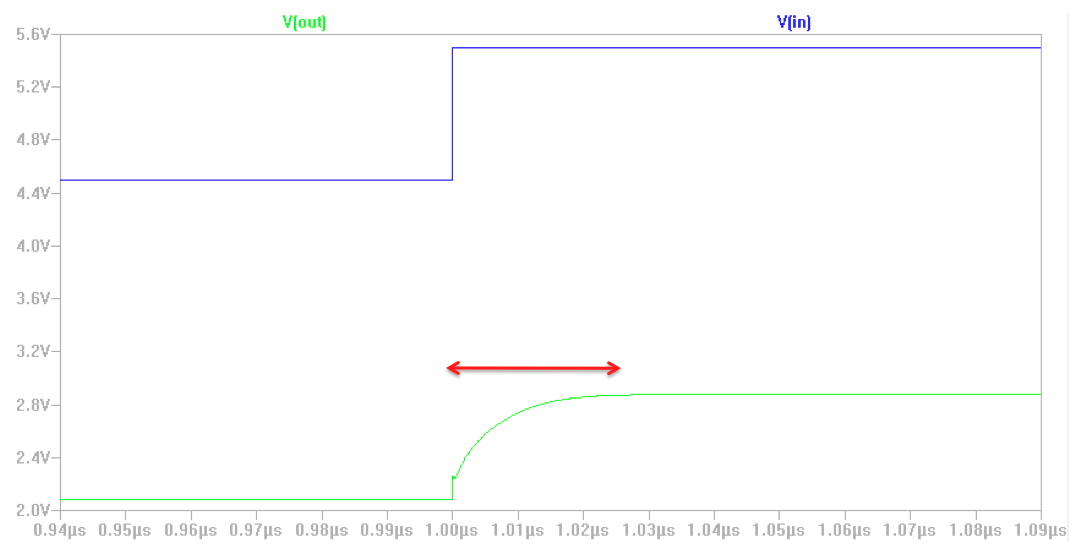
\includegraphics[width=4in]{Media/pos.png}
	\end{center}

	\begin{center}
		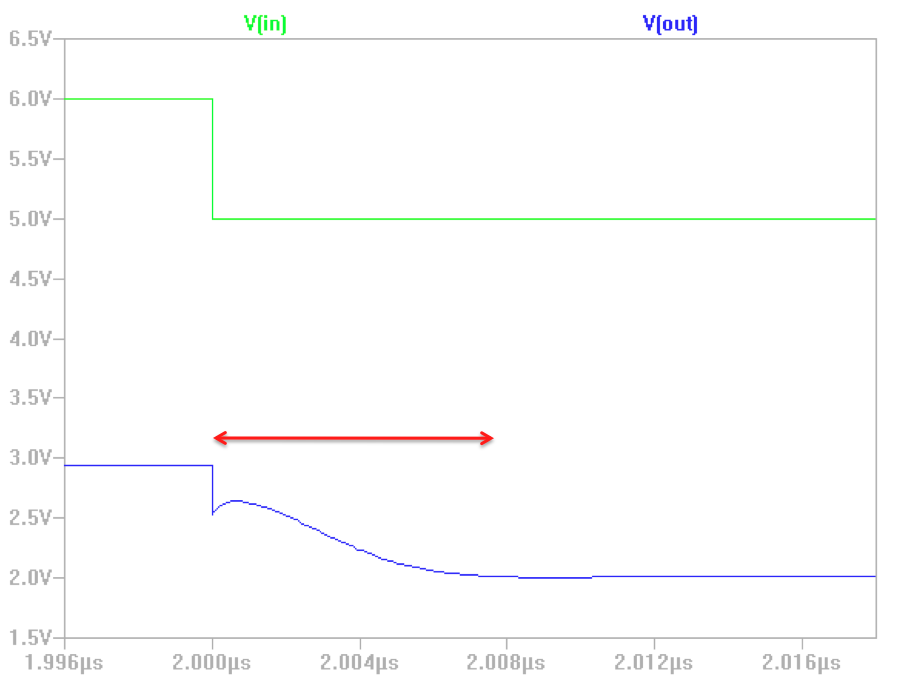
\includegraphics[width=4.0in]{Media/neg.png}
	\end{center}

Here is a temperature sweep of my regulator over a 35 degree Celsius range from 10 degrees Celcius to 45 degrees Celcius. It keeps the output without a 200 mV range of optimal. Outside of these temperatures performance is adversely affected.

\begin{figure}[h]
	\begin{center}
		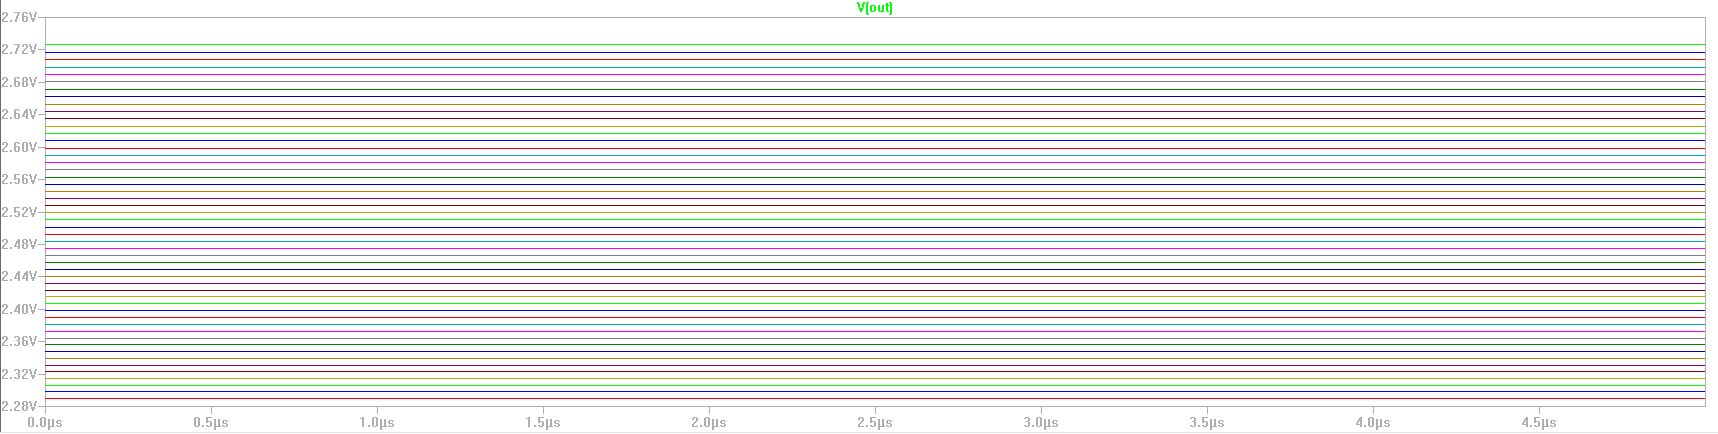
\includegraphics[width=3.5in]{Media/thermsw.png}
	\end{center}
	\caption{Regulator operation from 10 degrees C (top) to 45 degrees C (bottom) in 5 degree increments.}
	\label{fig:neg}
\end{figure}

%%%%%%%%%%%%%%%%%%%%%%%%%%%%%%%%%%%%%%%%%%%%%
\section{Layout}

I improved my op amp from homework 4 for this project. Here is my new op amp (the one I used above in simulations) as a schematic and also the layout for it.
	\begin{center}
		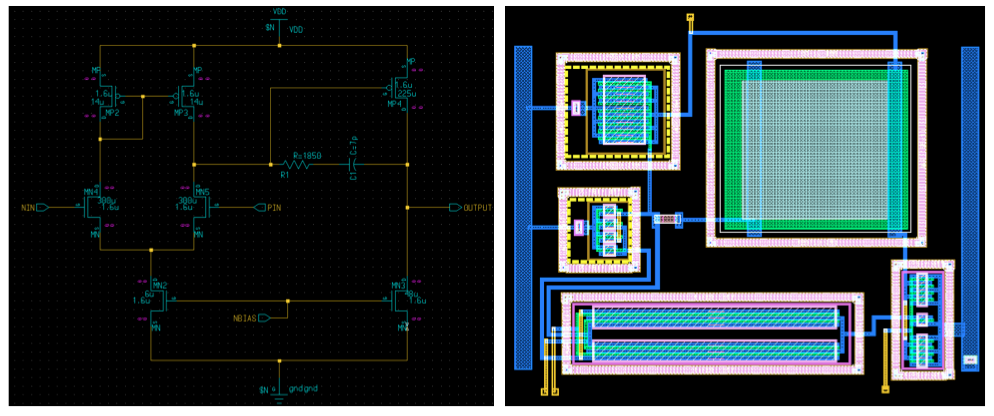
\includegraphics[width=7in]{Media/opamp.png}
	\end{center}

For the rest of my design, I have several resistors that I need to common centroid. Here is my common centroid scheme:

\begin{figure}[h]
	\begin{center}
		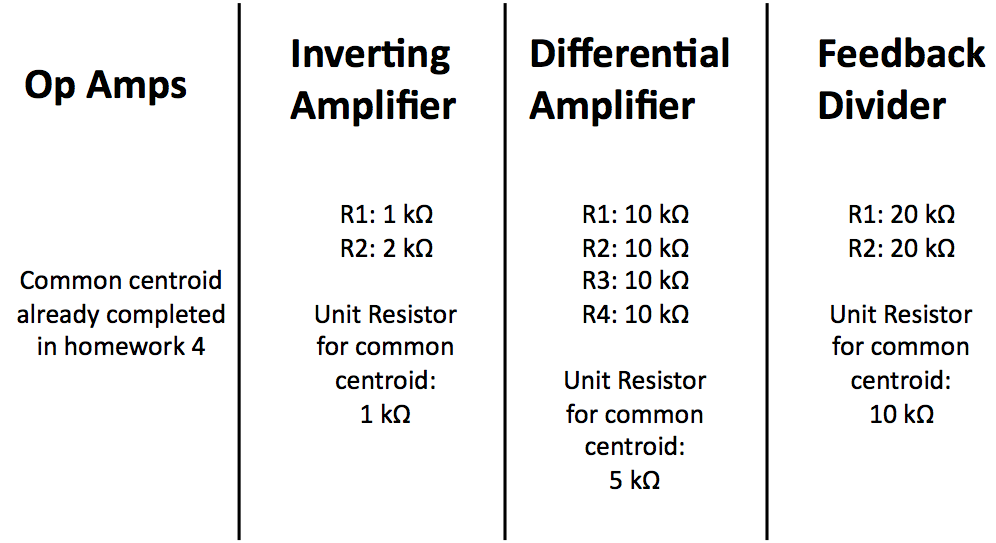
\includegraphics[width=4in]{Media/ccplan.png}
	\end{center}
	\caption{My common centroid scheme.}
	\label{fig:cc}
\end{figure}

\begin{figure}[h]
	\begin{center}
		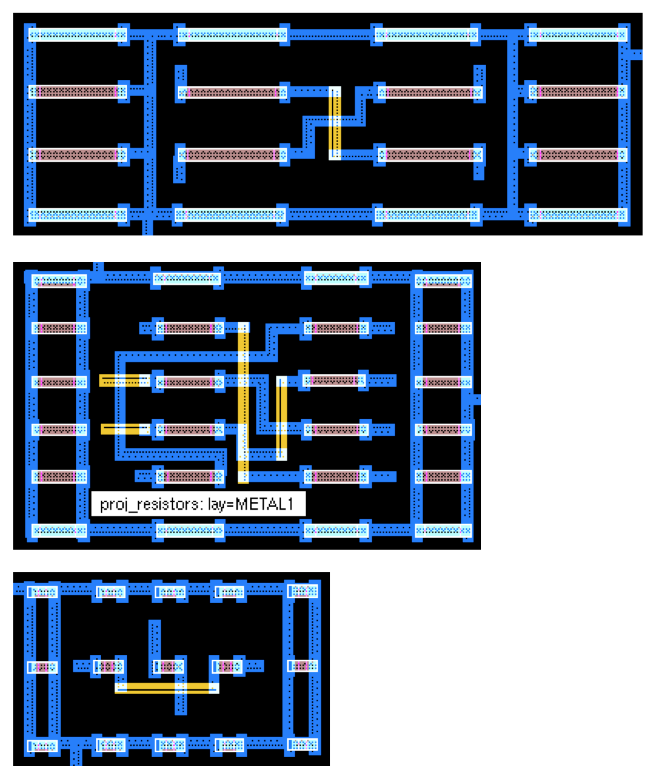
\includegraphics[width=4in, angle=90]{Media/res.png}
	\end{center}
	\caption{Common centroid resistors with dummy resistors added around the outside.}
	\label{fig:cc}
\end{figure}

\begin{figure}[H]
	\begin{center}
		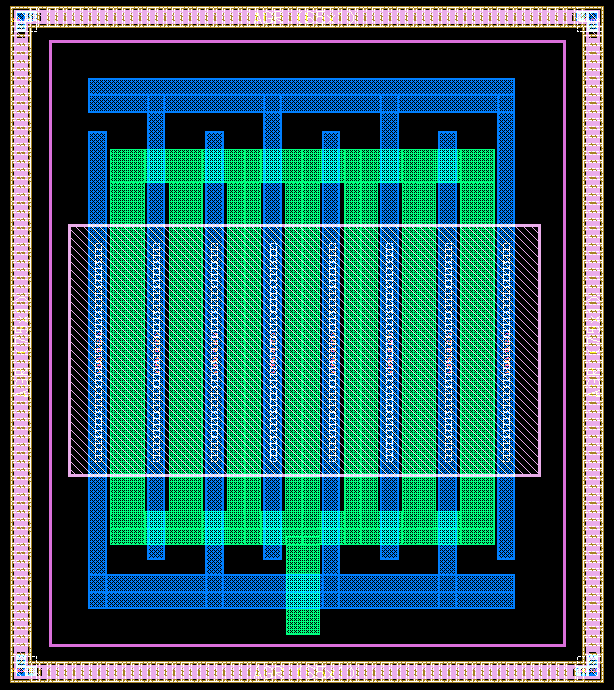
\includegraphics[width=4in, angle=90]{Media/lay_mos.png}
	\end{center}
	\caption{Power MOSFET. This is the pass element that controls power flow through the regulator.}
	\label{fig:cc}
\end{figure}

\begin{figure}[H]
	\begin{center}
		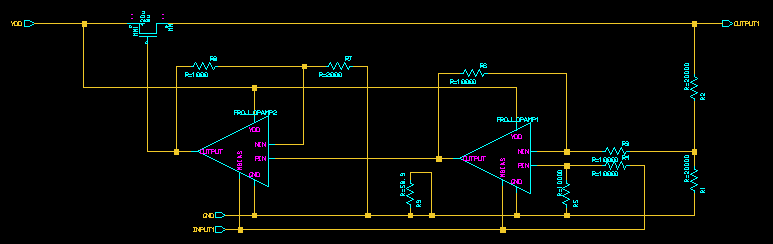
\includegraphics[width=5in]{Media/schem.png}
	\end{center}
	\caption{Final design in Design Architect.}
	\label{fig:cc}
\end{figure}

\begin{figure}[H]
	\begin{center}
		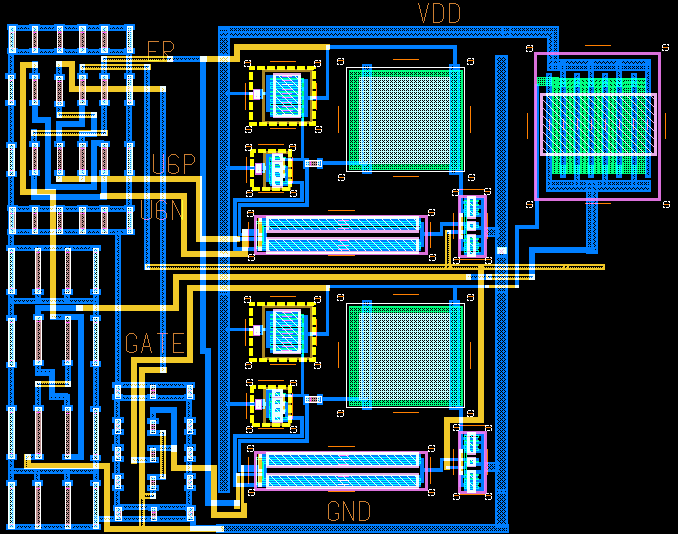
\includegraphics[width=8in, angle=90]{Media/lay_final.png}
	\end{center}
	\caption{Final Layout.}
	\label{fig:cc}
\end{figure}

\begin{figure}[H]
	\begin{center}
		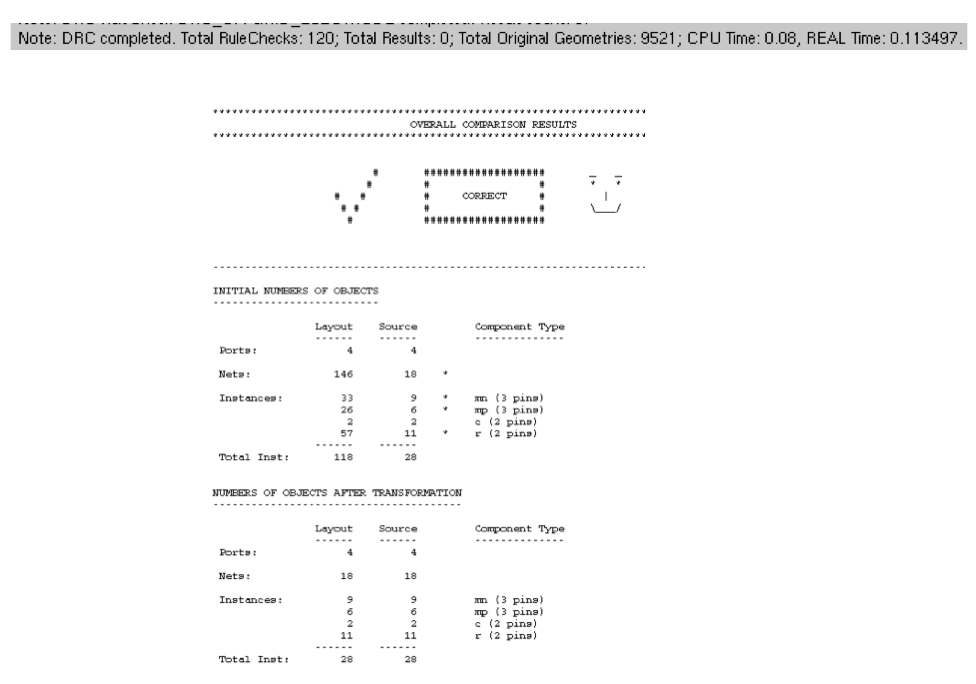
\includegraphics[width=6in]{Media/checks.png}
	\end{center}
	\caption{The design is DRC (top) and LVS (bottom) clean.}
	\label{fig:cc}
\end{figure}

\begin{figure}[H]
	\begin{center}
		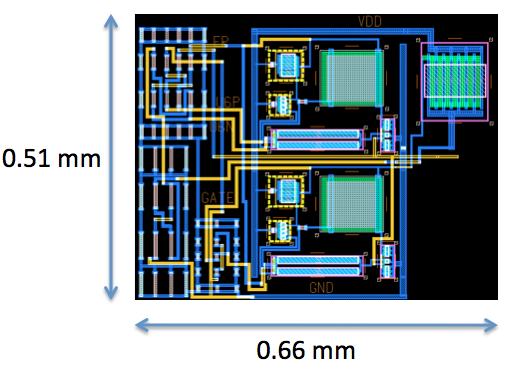
\includegraphics[width=3.5in]{Media/area.png}
	\end{center}
	\caption{The area is 0.33 mm$^2$.}
	\label{fig:cc}
\end{figure}

\end{document}



